\documentclass[11pt,a4paper,oneside]{book}

% Packages
\usepackage{assets/defpackages}
\usepackage{assets/mathcmd}
\usepackage{optionalcmd}
\usepackage{float}
\usepackage{indentfirst}

\usepackage[numbers]{natbib}
\usepackage[nottoc]{tocbibind}

\usepackage{lmodern}
\renewcommand*\familydefault{\sfdefault} %% Only if the base font of the document is to be sans serif
\usepackage[T1]{fontenc}
\usepackage{csquotes}
\MakeOuterQuote{"}

\graphicspath{{./components/images/}}

% Assets
\def\hmargin{18mm}
\def\vmargin{25mm}

%%% Tento soubor obsahuje definice různých užitečných maker a~prostředí %%%
%%% Další makra připisujte sem, ať nepřekáží v~ostatních souborech.     %%%

%%% Drobné úpravy stylu

% Tato makra přesvědčují mírně ošklivým trikem LaTeX, aby hlavičky kapitol
% sázel příčetněji a~nevynechával nad nimi spoustu místa. Směle ignorujte.
%\makeatletter
%\def\@makechapterhead#1{
%  {\parindent \z@ \raggedright \normalfont
%   \Huge\bfseries \thechapter. #1
%   \par\nobreak
%   \vskip 20\p@
%}}
%\def\@makeschapterhead#1{
%  {\parindent \z@ \raggedright \normalfont
%   \Huge\bfseries #1
%   \par\nobreak
%   \vskip 20\p@
%}}
%\makeatother

\setlength{\parskip}{0.3em}
\setlist{topsep=0.1em, itemsep=0em}

% Toto makro definuje kapitolu, která není očíslovaná, ale je uvedena v~obsahu.
\def\chapwithtoc#1{
\chapter*{#1}
\addcontentsline{toc}{chapter}{#1}
}

% Trochu volnější nastavení dělení slov, než je default.
\lefthyphenmin=2
\righthyphenmin=2

% Zapne černé "slimáky" na koncích řádků, které přetekly, abychom si
% jich lépe všimli.
\overfullrule=1mm

\renewenvironment{proof}[1][]{
  \par\medskip\noindent
  \textit{\ifthenelse{\equal{#1}{}}
  {Důkaz}
  {#1}}.
}{
\hspace*{\fill}$\qedsymbol$\par\medskip
}

\def\normalipe{0.8}

\newcommand{\exercisesolution}[3]{\textbf{\ref{exercise:ch#1_#2}}\quad #3.\\}
\geometry{
	top=\vmargin,
	bottom=\vmargin,
	left=\hmargin,
	right=\hmargin
}
\setlength{\parindent}{0pt}
\setlength{\parskip}{\baselineskip}

% Title page info
\def\maintitle{Základy středoškolské kombinatoriky}
\def\authorname{\textsc{David Weber}}
\def\email{david.weber99@seznam.cz}
\def\currentdate{\today}

\begin{document}
    
    % Title page
    \def\spacing{0.7em}
\def\bigspacing{5em}

\begin{titlepage}
    \begin{center}
        \vspace*{\fill}
        \Huge{\textbf{\maintitle}}\\
        \vspace*{\spacing}
        \Large{\authorname}\\
        \vspace*{\bigspacing}
        \vspace*{\fill}
        \large{\email}\\
        \vspace*{\spacing}
        \large{\currentdate}
    \end{center}
    \pagenumbering{arabic}
    \normalsize
\end{titlepage}

    \tableofcontents

    % Main content
    \chapter{Úvodem}

\section{Was ist kombinatorika?}

\textbf{Kombinatorika} představuje matematickou disciplínu zabývající se se kolekcemi prvků množin s definovanou vnitřní strukturou. Řekneme-li to méně formálně, studuje, kolika způsoby lze sestavit konfiguraci s jistými vlastnostmi. Zároveň se tak váže k blízkému oboru zvanému \textbf{teorie pravděpodobnosti}. \par
Typickou úlohou (otázkou) kombinatoriky je třeba tato:

\begin{exercise}
    Na svatbě je $n$ lidí.
    \begin{enumerate}[label=(\alph*)]
        \item Kolika způsoby lze $n$ svatebčanů sestavit do řady?
        \item V kolika případech stojí nevěsta napravo od ženicha?
        \item Kolik je řad, že ženich a nevěsta stojí vedle sebe?
    \end{enumerate}
\end{exercise}

Pro podobné úlohy v dalších odstavcích vybudujeme potřebný matematický aparát.
\section{Množiny}

Množiny pro nás budou klíčovým pojmem, neboť s jejich pomocí budeme formulovat další části výkladu. Proto považuji za nezbytné si zopakovat aspoň některé základní vlastnosti a operace, které s množinami můžeme provádět. Množinou v matematice rozumíme "soubor neuspořádaných prvků". Dvě množiny tak považujeme za stejné (sobě rovné) právě tehdy, když mají stejné prvky. Byť tento popis nepředstavuje zcela formální definici, pro naše potřeby s tímto chápáním vystačíme.\par
Množiny zapisujeme pomocí složených závorek $\{,\}$, přičemž jejich specifikace lze provést dvě způsoby:
\begin{itemize}
    \item výčtem (výpisem) jednotlivých prvků,
    \item společnou vlastností
\end{itemize}

\begin{example}
    Množinu $M$ obsahující prvky $a,\,b,\,c$ lze zapsat jako
    \begin{equation*}
        M=\set{a,\,b,\,c}.
    \end{equation*}
\end{example}
V případě většího počtu prvků, avšak s jistou strukturou, můžeme množinu specifikovat buď pomocí "\dots" nebo explicitním vyjádřením specifické vlastnosti.

\begin{example}
    Množinu všech přirozených čísel menších nebo rovny 5 lze zapsat jako
    \begin{equation*}
        S=\set{n\in\N \admid n \leqslant 5}\;\;\;\text{nebo}\;\;\;S=\set{1,\,2,\,\dots,\,5}.
    \end{equation*}
\end{example}

Důležitou vlastností množin je, že neuvažujeme násobné výskyty prvků. Tedy např. množiny $M=\set{1,\,2,\,3}$ a $N=\set{1,\,2,\,2,\,3,\,3}$ jsou si rovny, tj. $M=N$. Též je vhodné si připomenout, že chceme-li vyjádřit, že libovolný prvek $a$ je v množině $A$, pak píšeme $a \in A$ (čteme "$a$ náleží množině $A$"). Naopak v případě, že prvek $a$ nenáleží množině $A$, píšeme $a \notin A$.\par
Podstatnou vlastností pro nás budou operace \emph{sjednocení}, \emph{průniku} a \emph{rozdílu} množin.

\begin{definition}[Sjenocení, průnik a rozdíl]\label{def:mnozinove_operace}
    Mějme množiny\footnote{Mohou být \textbf{konečné} i \textbf{nekonečné}, avšak nás budou zajímat konečné množiny.} $A,\,B$. Pak definujeme:
    \begin{enumerate}[label=(\roman*)]
        \item sjednocení $A \cup B = \set{x \admid x\in A \lor x\in B}$, tj. výsledná množina obsahuje prvky množiny $A$ a zároveň prvky množiny $B$.
        \item průnik $A \cap B = \set{x \admid x\in A \land x\in B}$, tj. výsledná množina obsahuje \emph{pouze} prvky, které náleží oběma množinám.
        \item rozdíl $A \setminus B = \set{x \admid x\in A \land x \notin B}$, tj. výsledná množina obsahuje pouze ty prvky z množiny $A$, které nenáleží množině $B$.
    \end{enumerate}
\end{definition}

\begin{example}
    Pro množiny\footnote{U množiny $Y$ si uvědomme, že prvek $\set{z}$ není to samé jako prvek $z$, tedy např. po sjednocení se ve výsledné množině vyskytnou oba.} $X=\set{x,\,y,\,z}$ a $Y=\set{x,z,\set{z},w}$ platí
    \begin{itemize}
        \item $X \cup Y = \set{x,\,y,\,z} \cup \set{x,z,\set{z},w}=\set{x,\,y,\,z,\,x,z,\set{z},w}=\set{x,\,y,\,z,\,\set{z},w}$,
        \item $X \cap Y = \set{x,\,y,\,z} \cap \set{x,z,\set{z},w}=\set{x,\,z}$,
        \item $X \setminus Y = \set{x,\,y,\,z} \setminus \set{x,z,\set{z},w}=\set{y}$.
    \end{itemize}
    Zkuste si výsledky operací porovnat s definicí \ref{def:mnozinove_operace} výše.
\end{example}

Pro větší počet množin můžeme využít pro zápis sjednocení tzv. \emph{velké operátory} $\bigcup,\,\bigcap$. Máme-li tedy množiny $X_1,\,X_2,\,\dots,\,X_n$, můžeme jejich sjednocení, resp. průnik zapsat jako
\begin{equation*}
    \bigcup\limits_{i=1}^{n}X_i = X_1 \cup X_2 \cup \dots \cup X_n\;\;\;\text{resp.}\;\;\;\bigcap\limits_{i=1}^{n}X_i = X_1 \cap X_2 \cap \dots \cap X_n
\end{equation*}

Dále, co nás bude zajímat, je velkost množiny. Tu budeme označovat svislými čarami, tedy např. velikost množiny $X$ zapíšeme jako $\sizeof{X}$. Konkrétně např. pro množinu $A=\set{-1,\,0,10,20}$ je velikost $\sizeof{A}=4$.

\begin{remark}
    K závěru ještě pár poznámek:
    \begin{itemize}
        \item Prázdnou množinu (tj. množinu neobsahující žádné prvky) budeme značit symbolem $\emptyset$.
        \item Pokud platí pro množiny $A$ a $B$, že nemají žádné společné prvky, tj. $A \cap B=\emptyset$, pak je nazýváme \emph{disjunktní}. Obecněji řekneme-li, že množiny $X_1,\,X_2,\,\dots,\,X_n$ jsou \emph{\textbf{po dvou} disjunktní}, pak tím myslíme, že pro libovolnou dvojici množin $X_i$ a $X_j$ platí
        \begin{equation*}
            X_i \cap X_j = \emptyset,
        \end{equation*}
        přičemž $0 \leqslant i,\,j \leqslant n$.
    \end{itemize}
\end{remark}

Jako poslední zmíníme pojem tzv. \emph{podmnožiny}, který později využijeme hlavně v pravděpodobnosti.

\begin{definition}[Podmnožina]
    Mějme množiny $A$ a $B$. Řekneme, že množina $A$ je \textbf{podmnožinou} množiny $B$, pokud platí
    \[x\in A\implies x\in B.\]
    (Píšeme $A\subseteq B$.)
\end{definition}
    \chapter{Kombinatorické počítání}

Nyní se již podíváme na některé základní nástroje kombinatoriky a jejich využití. Na úvod se takto proto podíváme na pár motivačních příkladů.

\section{Pravidlo součinu a součtu}

Vezměme si pro začátek jednu motivační úlohu.

\begin{exercise}
    \textit{Předpokládejme, že chceme zjistit počet různých kurzů nabízených Wisconsinskou univerzitou v Madisonu. Kurzy rozdělíme podle oddělení, na kterém jsou uvedeny. Za předpokladu, že nedochází ke křížovému vypisování (křížové vypisování nastává, když je stejný kurz vypsán na více než jedné katedře), kolik předmětů si můžeme jako studenti zapsat?} \citep[str. 28]{Brualdi2018}
\end{exercise}

\begin{solution}\label{exercise:addition_principle}
    K problému můžeme přistoupit následovně: předměty si postupně rozdělíme do množin. Množinu všech dostupných předmětů si označíme $C$ (z angl. \emph{classes}). To znamená, že hledáme $\sizeof{C}$. Předměty si rozdělíme do množin podle katedry, která je nabízí. Tedy máme-li na univerzitě, pro zjednodušení, např. 5 kateder, pak se nám předměty rozdělí do pěti množin, které si označíme $C_1,\,\dots,\, C_5$. Množina všech předmětů $C$ je jednoduše sjednocením předmětů z jednotlivých kateder $C_1,\,\dots,\, C_5$, tj.
    \begin{equation*}
        C=\bigcup\limits_{i=1}^{5}C_i=C_1\cup C_2\cup C_3\cup C_4\cup C_5\,.
    \end{equation*}
    Protože ze zadání víme, že každý předmět je vypsán v rámci \textbf{právě jedné} katedry, pak množiny $C_1,\,\dots,\, C_5$ jsou po dvou disjunktní. Takže nám jednoduše stačí spočítat předměty na jednotlivých katedrách
    \begin{equation*}
        \sizeof{C}=\sum_{i=1}^{5}\sizeof{C_i}=\sizeof{C_1}+\sizeof{C_2}+\sizeof{C_3}+\sizeof{C_4}+\sizeof{C_5}\,.
    \end{equation*}
\end{solution}

Ačkoliv jsme úlohu \ref{exercise:addition_principle} jsme řešili sice trochu složitě, intuitivně je tento způsob nejspíše jasný. Máme-li $n_1$ způsobů, jak provést určitou akci a $n_2$ způsobů, jak provést nějakou jinou akci (kterou nelze provést současně s první), pak máme dohromady $n_1+n_2$ způsobů, jak vybrat některou činnost.\par
Z tohoto jednoduchého principu plyne tzv. \emph{kombinatorické pravidlo součtu}, které budeme v dalších úlohách využívat.

\begin{theorem}[Kombinatorické pravidlo součtu]\label{thm:pravidlo_souctu}
    Jsou-li $X_1,\,X_2,\,\dots,\,X_n$ konečné množiny, které jsou po dvou disjunktní, pak platí
    \begin{equation*}
        \sizeof{X_1\cup X_2\cup\dots\cup X_n}=\sizeof{X_1}+\sizeof{X_2}+\dots+\sizeof{X_n}
    \end{equation*}
    nebo zkráceně
    \begin{equation*}
        \sizeof{\bigcup\limits_{i=1}^{n}X_i}=\sum_{i=1}^{n}\sizeof{X_i}.
    \end{equation*}
\end{theorem}

Představme si, že máme městečka $A,\,B,\,C$, mezi nimiž vede po řadě 3 a 5 cest (tj. 3 cesty mezi $A$ a $B$, 4 cesty mezi $B$ a $C$).

\begin{figure}[H]
	\centering
	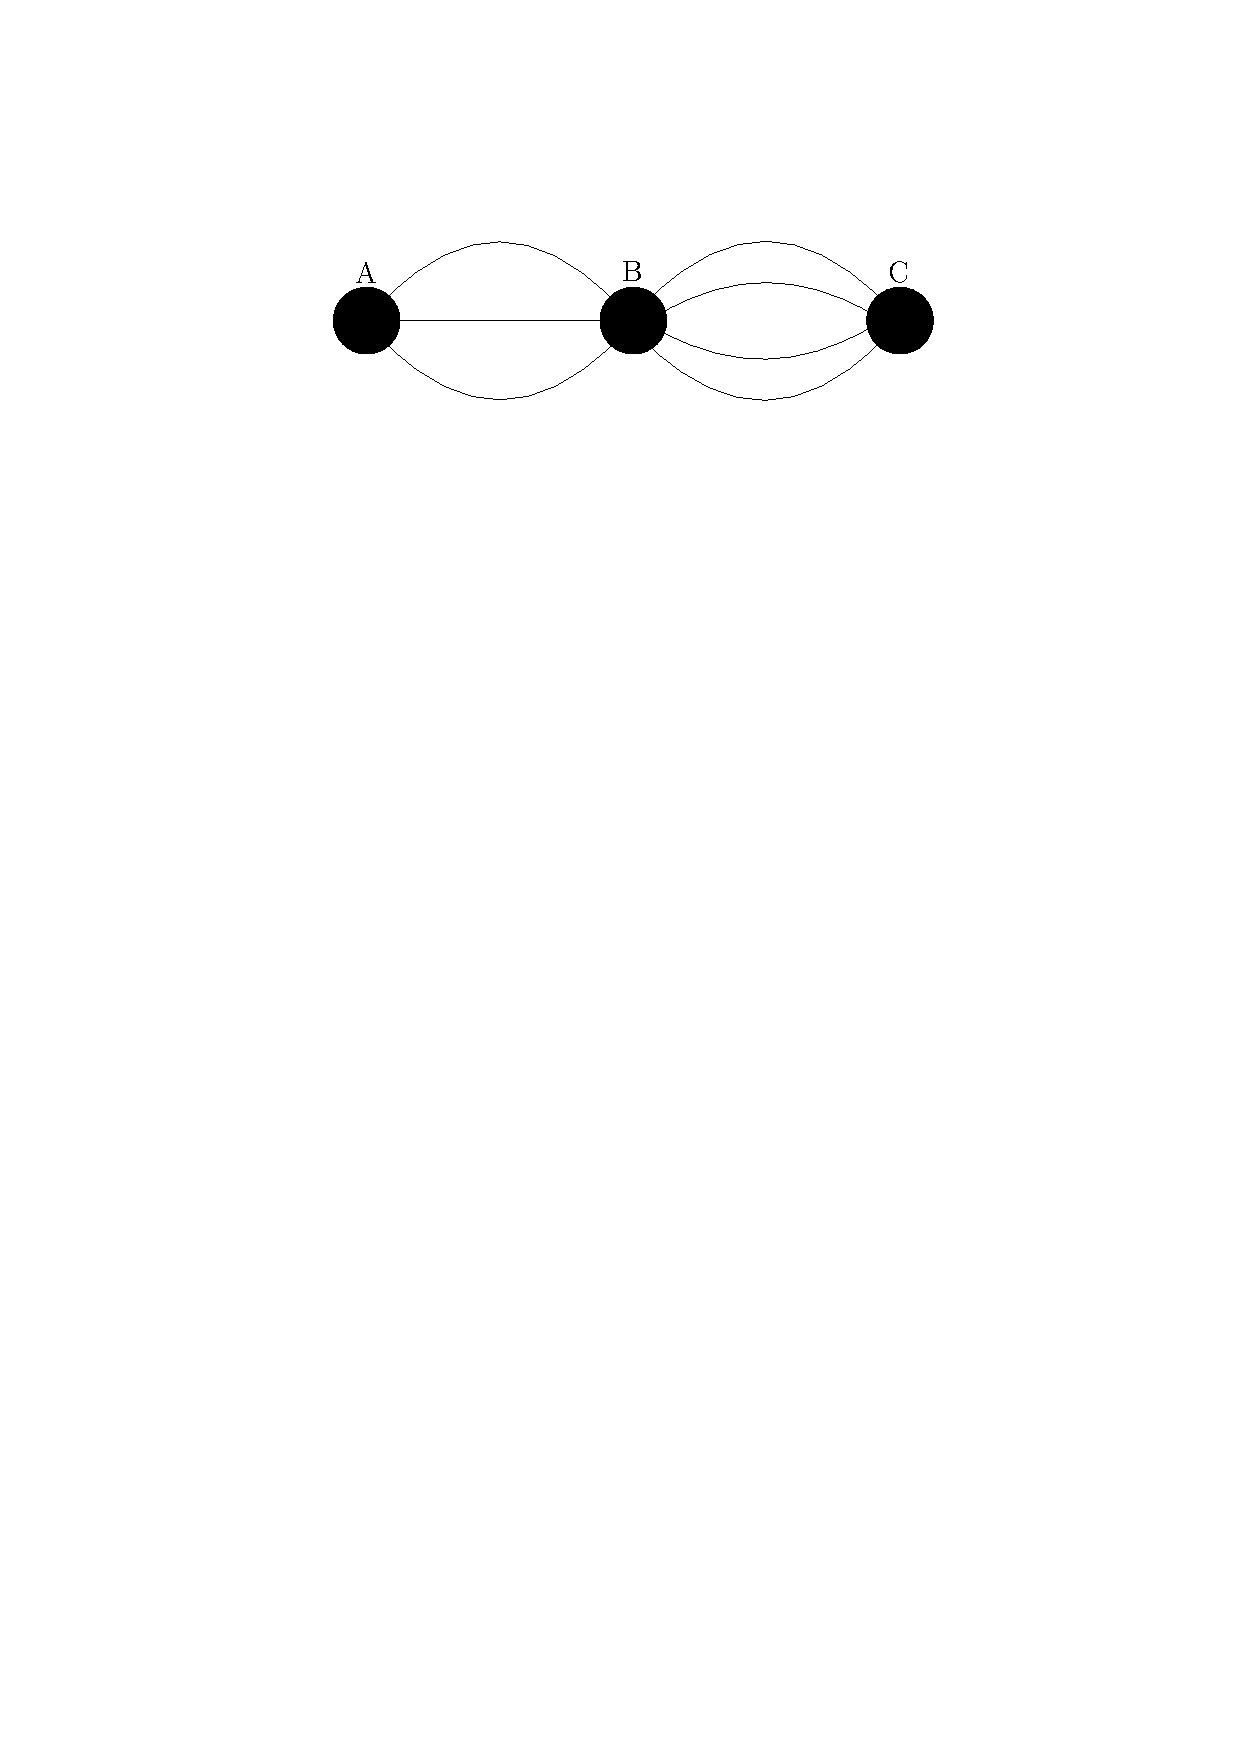
\includegraphics[scale=\normalipe]{ch02_mesta.pdf}
    \caption{Cesty mezi městy $A,\,B,\,C$.}
    \label{fig:mesta}
\end{figure}

Chceme zjistit počet všech způsobů, jak se dostat z města $A$ do města $C$. Jak aplikujeme pravidlo součtu zde? Mohli bychom si zde rozdělit cesty z $A$ do $C$ do množin podle toho, kterou cestou jsme dorazili z $A$ do $B$. Pokud tak učiníme, pak jsme rozdělili cesty do celkem tří množin $P_1,\,P_2,\,P_3$, přičemž všechny jsou po dvou disjunktní (žádná z cest z $A$ do $C$ nemůže obsahovat dvě různé cesty z $A$ do $B$) a množina $P$ obsahuje všechny cesty z $A$ do $C$. Tedy celkový počet cest $\sizeof{P}$ je roven součtu $\sizeof{P_1}+\sizeof{P_2}+\sizeof{P_3}$. Pro každou cestu mezi městy $A$ a $B$ máme 4 možnosti, kudy se dostat z $B$ do $C$. Tedy
\begin{equation*}
    \sizeof{P_1}=\sizeof{P_2}=\sizeof{P_3}=4.
\end{equation*}
To znamená, že celkový počet cest $\sizeof{P}=\sizeof{P_1}+\sizeof{P_2}+\sizeof{P_3}=4+4+4=3\cdot 4=12.$.\par
Tento způsob je jistě velmi nepraktický a navíc je celkem očividné, že na daný výsledek jsme mohli přijít hned. Stačilo vynásobit počet cest mezi městy $A$ a $B$ a počet cest mezi městy $B$ a $C$. Z toho dostáváme druhé kombinatorické pravidlo:

\begin{theorem}[Kombinatorické pravidlo součinu]\label{thm:pravidlo_soucinu}
    Počet uspořádaných $k$-tic, jejichž $i$-tý člen lze vybrat $n_i$ způsoby je roven
    \begin{equation*}
        n_1\cdot n_2\cdot\dots\cdot n_k = \prod_{i=1}^{k}n_i
    \end{equation*}
\end{theorem}
Je důležité zmínit, že jednotlivé výběry \textbf{musí být nezávislé}, tedy výběr na jednu pozici nesmí ovlivnit počet výběrů na ostatní pozice. Méně formálně, avšak užitečněji, můžeme pravidlo formulovat i takto: \textit{Lze-li první výběr provést celkem $n$ způsoby a druhý výběr $m$ způsoby bez ohledu na první výběr, pak celkový počet dvojic možných výběrů je $nm$.} (Pochopitelně, toto lze zobecnit na libovolný počet výběrů, jako je tomu v \ref{thm:pravidlo_soucinu}.)

\begin{exercise}
    Křídy jsou vyráběny
    \begin{itemize}
        \item ve 3 různých barvách,
        \item v 8 různých délkách
        \item a o 4 různých průměrech.
    \end{itemize}
    Kolik typů kříd celkově lze zakoupit? \citep[str. 29]{Brualdi2018}
\end{exercise}
\begin{solution}
    Barvu křídy můžeme vybrat celkem třemi způsoby, délku osmi způsoby a průměr křídy celkem čtyřmi způsoby. Protože výběry jsou na sobě nezávislé, pak podle předchozího pravidla součinu existuje celkem $3\cdot 8\cdot 4=96$ typů kříd.
\end{solution}

\begin{exercise}
    Kolik čtyřciferných přirozených čísel lze sestavit z cifer 0, 1, 2, 3, 4, 5, jestliže
    \begin{enumerate}[label=(\alph*)]
        \item cifry se mohou opakovat,
        \item cifry se nemohou opakovat?
    \end{enumerate}
    (Úloha i řešení \citep[str. 7]{Slavik2022}.)
\end{exercise}
\begin{solution}{Řešení (a)}
    Protože se cifry mohou opakovat, pak na každé číselné pozici máme stejný počet možností výběru číslici, až na první pozici, neboť nemůžeme vybrat číslici 0 (jinak by se nejednalo o \emph{čtyřciferné} číslo). Na první pozici máme tak 5 možností výběru a na zbylých třech máme 6 možností, tj. celkově existuje
    \begin{equation*}
        5\cdot 6\cdot 6\cdot 6 = 1080\;\text{možností.}
    \end{equation*}
\end{solution}
\begin{solution}{Řešení (b)}
    Tentokrát se cifry nesmí opakovat. Úvaha tak zůstává stejná, ale při určování počtu možností výběru musíme zohlednit již vybrané číslice. Na první pozici tak máme 5 možností výběru (nesmíme vybrat nulu), na druhé pozici máme 5 možností (původně jsme měli 6, ale jednu cifru jsme již použili na první pozici), na třetí pozici máme 4 možnosti (2 číslice jsme již použili) a na čtvrté pozici máme 3 možnosti. Celkově tak existuje
    \begin{equation*}
        5\cdot 5\cdot 4\cdot 3=300\;\text{možností.}
    \end{equation*}
\end{solution}

Kombinatorické pravidlo součtu a součinu však můžeme v různých úlohách kombinovat. Speciálně, pokud si tak ulehčíme hledání určených konfigurací.

\begin{exercise}
    Kolik sudých čísel čtyřciferných přirozených čísel lze sestavit z cifer 0, 1, 2, 3, 4, 5, jestliže se nesmí opakovat? (Úloha i řešení \citep[str. 8]{Slavik2022}.)
\end{exercise}
\begin{solution}
    Aby výsledné číslo bylo sudé, musí končit (tj. mít na čtvrté pozici) číslici 0, 2, nebo 4. Zde již však nastává problém, neboť nemůžeme hned aplikovat pravidlo součinu. Je tomu tak proto, že pokud by byla na čtvrté pozici nula, pak na první pozici máme 5 možností, zatímco pokud by zde byla číslice 2, nebo 4, pak počet přípustných číslic na první pozici je již pouze 4 (nesmíme vybrat číslici 0 a pak číslici na čtvrté pozici). Počet výběrů tak již není nezávislý. Nicméně můžeme každý z případů vyšetřit zvlášť:
    \begin{itemize}
        \item označme si množinu $D_1$ (z angl. \emph{digit}) obsahující všechna čísla končící číslicí 0,
        \item množinu čísel $D_2$ končících číslicí 2 a
        \item množinu čísel $D_3$ končících číslicí 4.
    \end{itemize}
    Pro čísla končící nulou máme na první pozici celkem 5 možností, na druhé pak 4 možnosti a na třetí 3 možnosti. Tedy z kombinatorického pravidla součinu máme
    \begin{equation*}
        \sizeof{D_1}=5\cdot 4\cdot 3=60\;\text{možností.}
    \end{equation*}
    Množiny $D_2$ a $D_3$ mají stejnou velikost, neboť v obou případech máme na první pozici 4 možnosti výběru, na druhé 4 možnosti výběru a na třetí 3 možnosti. Tj.
    \begin{equation*}
        \sizeof{D_2}=\sizeof{D_3}=4\cdot 4\cdot 3=48\;\text{možností.}
    \end{equation*}
    Je jasné, že tyto množiny jsou disjunktní (každá dvojice množin obsahuje čísla s jinou číslicí na čtvrté pozici). Tedy podle kombinatorického principu součtu platí
    \begin{equation*}
        \sizeof{D_1\cup D_2\cup D_3}=\sizeof{D_1}+\sizeof{D_2}+\sizeof{D_3}=60+48+48=156\;\text{možností.}
    \end{equation*}
\end{solution}
\section{Variace, permutace a kombinace}

Nyní trochu rozšíříme na repertoár nástrojů. Zatím jsme řešili úlohy, kde jsme vybírali vždy "po jednom" prvku, abychom dosáhli jisté konfigurace. Nyní se podíváme, jakých výsledků dosáhneme v případě, kdy budeme již vybírat nějaké $k$-tice z nějaké $n$ prvkové množiny objektů.\par
Je třeba si rozmyslet dva základní případy:
\begin{itemize}
    \item výběr $k$-tic, kde \textbf{záleží na pořadí},
    \item výběr $k$-tic, kde \textbf{nezáleží na pořadí}.
\end{itemize}
S prvním případem jsme již do jisté míry obeznámeni, neboť u úloh, které jsme řešili, vždy záleželo na pořadí. To tedy vede na sestavování tzv. \emph{uspořádaných $k$-tic}, které jsme již zmínili ve formulaci kombinatorického pravidla součinu \ref{thm:pravidlo_soucinu}. Těm říkáme tzv. \textbf{variace $k$-té třídy z $n$ prvků}. Tedy např. variací 2. třídy z množiny $\set{1,\,2,\,3}$ je třeba
\begin{equation*}
    (1,\,3)\;\;\;\text{nebo}\;\;\;(3,\,1).
\end{equation*}

Druhý případ je pro nás novinkou. Vybíráme totiž tzv. \emph{neuspořádané $k$-tice}, tzn. vybereme-li např. z množiny $\set{a,\,b,\,c}$ neuspořádanou dvojici sestávající z prvků $a$ a $c$, pak je to stejné jako výběr neuspořádané dvojice sestávající z prvků $c$ a $a$. Takový výběr nazýváme \textbf{kombinací $k$-té třídy z $n$ prvků}.

Zatím se omezíme na tzv. variace, resp. kombinace \textbf{bez opakování}.

\subsection{Výběry bez opakování}

Výběrem bez opakování rozumíme výběr $k$-tice prvků takové, že se v ní žádný prvek neopakuje, tzn. každý je v ní nejvýše jednou. Tedy rozlišujeme
\begin{itemize}
    \item \emph{variace bez opakování} a
    \item \emph{kombinace bez opakování}.
\end{itemize}
Pojďme se nyní podívat na metody jejich výpočtu.

\begin{theorem}[Variace bez opakování]\label{thm:variace_bez_opakovani}
    Počet uspořádaných $k$-tic sestavených z $n$-prvkové množiny tak, že se každý prvek ve výběru vyskytne nejvýše jednou, je roven
    \begin{equation*}
        \prod_{i=1}^{k}(n-i+1)=n(n-1)(n-2)\cdots(n-k+1).
    \end{equation*}
\end{theorem}
\begin{proof}
    Tento fakt přímo plyne z kombinatorického pravidla součinu. Na první pozici máme $n$ možností výběru, na druhé $n-1$ možností, \dots a pro $k$-tý člen máme $n-k+1$ možností. Tedy celkově $n(n-1)\cdots(n-k+1)$ možností.
\end{proof}

Počet variací $k$-té třídy z $n$-prvkové množiny bez opakování budeme značit $V_k(n)$.

\begin{exercise}
    Ve třídě, kde je celkem 25 dětí, si žáci volí nového pokladníka, šatnáře a službu na tabuli, přičemž jeden žák nesmí zastávat více pozic zároveň. Kolika různými způsoby si může třída zvolit žáky na dané pozice.
\end{exercise}
\begin{solution}
    V tomto případě jistě záleží na pořadí výběru (vybrat žáka na pozici šatnáře není jistě to samé, jako jej vybrat na pozici pokladníka). Tedy budeme počítat variace 3. třídy z 25 prvků bez opakování, tedy existuje
    \begin{equation*}
        V_3(25)\stackrel{\ref{thm:variace_bez_opakovani}}{=}25\cdot(25-1)\cdot(25-2)=25\cdot 24\cdot 23=13 800\;\text{způsobů.}
    \end{equation*}
\end{solution}

Dalším důležitým, a zatím nezmíněným termínem, je tzv. \emph{permutace}. Permutací rozumíme libovolné uspořádání $n$ prvků do řady. Tedy např. 5, 3, 2, 4, 1 je permutace množiny $\set{1,\,2,\,3,\,4,\,5}$. Permutace lze interpretovat jako uspořádané $n$-tice, což z nich dělá speciální případ variace (výběr uspořádané $n$-tice z $n$ prvkové množiny). Stejně jako u variací a kombinací rozlišujeme permutace s opakováním a bez opakování.
\begin{theorem}[Permutace bez opakování]
    Počet uspořádaných $n$-tic z $n$-prvkové množiny tak, že se každý prvek ve výběru vyskytne nejvýše jednou, je
    \begin{equation*}
        \prod_{i=1}^{n}i=n(n-1)(n-2)\dots 2\cdot 1.
    \end{equation*}
\end{theorem}
\begin{proof}
    Permutace je speciálním případem variace pro $k=n$, tedy $V_n(n)\stackrel{\ref{thm:variace_bez_opakovani}}{=}n(n-1)(n-2)\cdots 2\cdot 1$.
\end{proof}

\begin{definition}[Faktoriál]
    Je-li $n\in\N$, pak definujeme číslo
    \begin{equation*}
        n!=n(n-1)(n-2)\cdots 2\cdot 1=\prod_{i=1}^{n}i,
    \end{equation*}
    které nazýváme \emph{faktoriál} (čteme "$n$ faktoriál").
\end{definition}

Číslo $n!$ tedy vyjadřuje počet permutací $n$ prvkové množiny\footnote{Podobně jako pro variace, i pro permutaci $n$ prvkové množiny se zřídka používá značení $P(n)$. Avšak je tomu tak málokdy, neboť často se při výpočtech píše rovnou $n!$.}.

\begin{exercise}
    Z 10 knih je 6 psáno česky a zbylé 4 latinsky. Kolika různými způsoby lze daná knihy umístit na poličku, jestliže všechny knihy psané česky mají být vedle sebe a všechny latinsky psané vedle sebe?\cite{Havrlant2022}
\end{exercise}
\begin{solution}
    Všechny české knihy chceme seřadit vedle sebe, tj. jedná se o permutaci na šesti prvcích, kterých je $6!$. Podobně latinsky psané knihy lze vedle sebe seřadit $4!$ způsoby. Seřazení český a latinských knih jsou na sobě nezávislá a tedy podle kombinatorického pravidla součinu existuje
    \begin{equation*}
        6!\cdot 4!=(6\cdot 5\cdot 4\cdot 3\cdot 2\cdot 1)\cdot(4\cdot 3\cdot 2\cdot 1)=720\cdot 24=17 280\;\text{možností.}
    \end{equation*}
\end{solution}

Zatím jsme se zabývali uspořádanými $k$-ticemi (variace a permutace), jejichž důležitou vlastností bylo, že záleželo na pořadí. Pokud ovšem chceme od pořadí upustit a soustředit se jen na vybrané prvky, budeme muset náš výpočet lehce upravit.

\begin{theorem}[Kombinace bez opakování]\label{thm:kombinace_bez_opakovani}
    Počet neuspořádaných $k$-tic sestavených z prvků $n$ prvkové množiny tak, že se každý prvek ve výběru vyskytne nejvýše jednou, je roven
    \begin{equation*}
        \dfrac{n(n-1)(n-2)\cdots(n-k+1)}{k!}=\dfrac{1}{k!}\prod_{i=1}^{k}(n-i+1)
    \end{equation*}
\end{theorem}
\begin{proof}
    Naši úvahu můžeme založit na následujícím pozorování: máme-li nějakou \emph{neuspořádanou} $k$-tici prvků z $n$ prvkové množiny, pak existuje přesně $k!$ způsobů, jak vybrané prvky uspořádat do řady, čímž z ní vytvoříme \emph{uspořádanou} $k$-tici. To znamená, že platí
    \begin{equation*}
        (\text{počet uspořádaných $k$-tic})=k!\cdot(\text{počet neuspořádaných $k$-tic}).
    \end{equation*}
    Počet neuspořádaných $k$-tic umíme vypočítat podle věty \ref{thm:variace_bez_opakovani}, tedy máme
    \begin{equation*}
        \prod_{i=1}^{k}(n-i+1)=k!\cdot(\text{počet neuspořádaných $k$-tic}).
    \end{equation*}
    Vydělíme-li rovnost číslem $k!$, dostaneme požadovaný výraz, tj.
    \begin{equation*}
        (\text{počet neuspořádaných $k$-tic})=\dfrac{1}{k!}\prod_{i=1}^{k}(n-i+1)
    \end{equation*}
\end{proof}
\section{Cvičení}

\begin{exercise}\label{exercise:ch02_1}
    \textit{Jana má pět různě barevných triček a tři nestejné sukně. Kolika způsoby si může vzít tričko a sukni, aby pokaždé vypadala jinak?} \citep[str. 145]{Petakova2020}
\end{exercise}
\begin{exercise}\label{exercise:ch02_2}
    V jedné třídě, ve které každý žák ovládá aspoň jeden ze dvou jazyků (angličtinu nebo němčinu), hovoří 25 žáků anglicky, 16 žáků německy a 7 žáků hovoří oběma jazyky. Kolik žáků chodí do této třídy? \citep[sekce Kombinatorika]{kdm2022}
\end{exercise}
\begin{exercise}\label{exercise:ch02_3}
    Určete počet všech přirozených čísel větších než 2000, v jejichž zápisech se vyskytují cifry 1, 2, 4, 6, 8, a to každá nejvýše jednou? \citep[str. 146]{Petakova2020}
\end{exercise}
\begin{exercise}\label{exercise:ch02_4}
    Na běžecké trati běží 8 závodníků. Za předpokladu, že každou z medailí získá právě jeden závodník, vypočítejte, kolik je možností na rozdělení zlaté, stříbrné a bronzové medaile mezi závodníky. \citep[str. 146]{Petakova2020}
\end{exercise}
\begin{exercise}\label{exercise:ch02_5}
    Ve třídě je 30 míst, ale ve třídě 3. B je pouze 28 žáků. Kolika způsoby lze sestavit zasedací pořádek? \citep[str. 146]{Petakova2020}
\end{exercise}
\begin{exercise}\label{exercise:ch02_6}
    Z kolika prvků lze vytvořit 992 variací druhé třídy bez opakování? \citep[str. 146]{Petakova2020}
\end{exercise}
\begin{exercise}\label{exercise:ch02_7}
    Kolika způsoby lze rozmíchat hru 32 karet? \citep[str. 146]{Petakova2020}
\end{exercise}
\begin{exercise}\label{exercise:ch02_8}
    Kolik různých devíticiferných čísel s různými ciframi lze sestavit z cifer 1 až 9? \citep[str. 146]{Petakova2020}
\end{exercise}
\begin{exercise}\label{exercise:ch02_9}
    Kolik přímek určuje deset různých bodů v rovině, z nichž
    \begin{enumerate}[label=(\alph*)]
        \item žádné tři neleží na jedná přímce,
        \item právě šest leží na jedné přímce?
    \end{enumerate}
    \citep[str. 146]{Petakova2020}
\end{exercise}
\begin{exercise}\label{exercise:ch02_10}
    Určete počet všech úhlopříček v konvexním mnohoúhelníku. \citep[str. 147]{Petakova2020}
\end{exercise}
\begin{exercise}\label{exercise:ch02_11}
    V krabici je 10 výrobků, z nichž jsou právě tři vadné. Kolika způsoby lze vybrat 5 výrobků tak, aby:
    \begin{enumerate}[label=(\alph*)]
        \item žádný nebyl vadný,
        \item právě jeden byl vadný,
        \item nejvýše jeden byl vadný,
        \item alespoň dva byly vadné.
    \end{enumerate}
    \citep[str. 147]{Petakova2020}
\end{exercise}
\begin{exercise}\label{exercise:ch02_12}
    Z kolika prvků lze vytvořit 990 kombinací druhé třídy bez opakování? \citep[str. 147]{Petakova2020}
\end{exercise}
\begin{exercise}\label{exercise:ch02_13}
    Učitel chce vytvořit ze čtyř dívek a čtyř chlapců jeden tříčlenný tým, v němž bude jedna dívka a dva chlapci. Kolika různými způsoby může sestavit tým? \citep[příklad \emph{Tříčlenné 69274}]{hackmath2022}
\end{exercise}

    % Bibliography
    
    \renewcommand{\bibname}{Seznam použité literatury}

    % \bibliographystyle{plainnat}    %% Autor (rok) s anglickými spojkami
    \bibliographystyle{unsrtnat}       %% [číslo]
    % \bibliographystyle{alpha}

    %%% Vytvoření seznamu literatury. Pozor, pokud jste necitovali ani jednu
    %%% položku, seznam se automaticky vynechá.
    \bibliography{components/bibliography.bib}

\end{document}